\documentclass{article}
\usepackage{graphicx}
\usepackage[margin=1.5cm]{geometry}
\usepackage{amsmath}
\usepackage{hyperref}

\begin{document}

\title{PhET Activity and Laboratory Measurements}
\author{Prof. Jordan C. Hanson}

\maketitle

\section{Theoretical Calculutions}

\begin{enumerate}
\item (With professor): We will show that, according to Newton's 2nd Law, that the motion of a \textit{pendulum} (Fig. \ref{fig:pendulum} obeys the following equation:
\begin{equation}
x(t) = a\cos(\omega t + \phi) \label{eq:1}
\end{equation} 
In Eq. \ref{eq:1}, $a$ is the amplitude in units of distance, $\omega$ is the angular frequency in units of radians per second, and $\phi$ is the phase in units of radians.  A fact that follows from Eq. \ref{eq:1} is that the period $T$ of the pendulum is related to the gravitational constant $g$ and pendulum $L$: $T = 2\pi \sqrt{L/g}$.
\begin{figure}[ht]
\centering
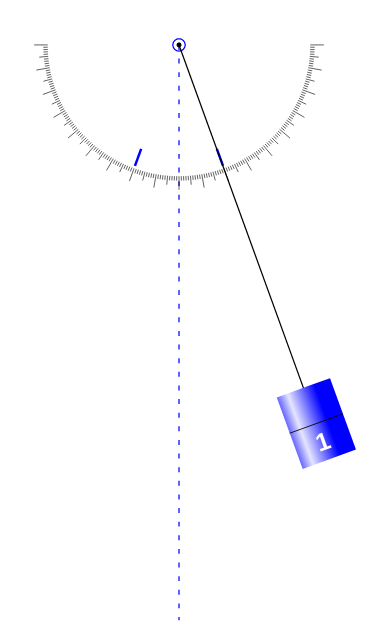
\includegraphics[width=0.2\textwidth]{pendulum.png}
\caption{\label{fig:pendulum} A pendulum is a mass $m$ that swings on a chord of length $L$ with angular frequency $\omega = \sqrt{g/L}$, where $g$ is the gravitational constant.}
\end{figure}
\item Point your browser to the following link: \url{https://phet.colorado.edu/en/simulations/pendulum-lab}.  Using the Intro tab of this PhET, create a data table of the \textit{period} of the pendulum in seconds, versus the \textit{length} in centimeters.  Create a graph of your data.  Do you recognize a pattern?  Using Excel, LibreOffice Calc, or Google Sheets to fit a polynomial to the simulated data.
\end{enumerate}

\section{Lab Measurement}

\begin{enumerate}
\item Using the communal pendulum set up for the class, we \textit{collect the same data we collected with the simulation.}
\item Create the same graph of the data from the real system alongside your graph of the simulated data.
\item Finally, graph the simulated period versus the square root of the length.  Do you notice a pattern?  Repeat this with the real data, and determine if the pattern holds in reality.
\end{enumerate}

\end{document}
